72. а) $f(x)=(x+1)|x-1|=\begin{cases}x^2-1,\ x\geqslant1,\\ 1-x^2,\ x<1.\end{cases}$
$$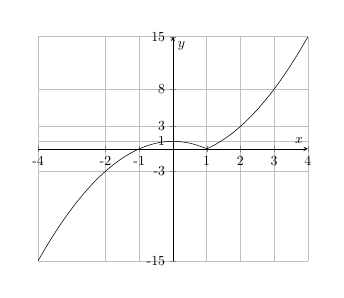
\begin{tikzpicture}[scale=0.5]
\begin{axis}[
    axis lines = middle,
    grid=major,
    legend pos={south west},
    xlabel = {$x$},
    ylabel = {$y$},
    ymin=-15,
    ymax=15,
    xmin=-4,
    xtick={-4,-2,1,4,3,2,-1},
    xticklabels={-4,-2,1,4,3,2,-1},
    ytick={ -15, -3,15,8,1,3},
    yticklabels={-15, -3,15,8,1,3}           ]
	\addplot[domain=-4:4, samples=100, color=black] {(x+1)*abs(x-1)};
%\addplot[domain=-4:3, samples=100, color=black] {abs(x*x-x-6)*(x-4)/(3-x)};
%\addplot[domain=-3:5, samples=100, color=black] {-abs(x-1)};
%\addplot[domain=-3.1:2.5, samples=100, color=red] {70*abs(1-2*abs(abs(x)-2))-10*x^2+10*x-70};
	%\addlegendentry{$\text{Рис. 1}$};
\end{axis}
%\draw (4.8,2.7) circle (2pt);
%\draw (4.8,5.2) circle (2pt);
\end{tikzpicture}$$
б) Исходя из графика, найдём ответ: функция возрастает при $x\in(-\infty;0]$ и $[1;+\infty),$ функция принимает положительные значения при $x\in(-1;1)\cup(1;+\infty),$ уравнение $f(x)=c$ имеет 3 решения при $c\in(0;1).$\\
